\subsection{Thermal Sunyaev-Zel'dovich data}
\label{sec:tsz_data}
    	\begin{figure}
	\centering
	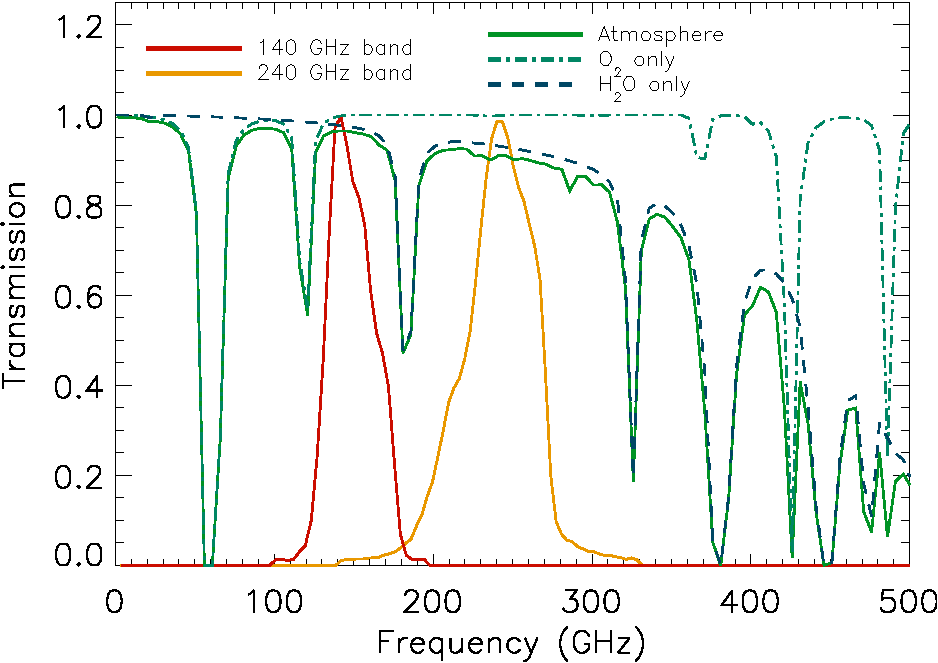
\includegraphics[width=\columnwidth]{Figure/bandpass}
	\caption{Normalized 140~GHz (solid red line) and 240~GHz (solid orange line) instrumental bandpasses. The total atmospheric transmission is also given as a solid green line for 1~mm of precipitable water vapor, according to the Pardo model \citep{Pardo}. The oxygen (dash-dotted light blue) and the water vapor (dashed dark blue) contributions are represented.}
        \label{fig:bandpass}
	\end{figure}
	
In the non-relativistic limit, the tSZ effect results in a distortion of the CMB black-body spectrum, whose intensity frequency dependence is given by \citep{Birkinshaw}
\begin{equation}
	g(x) = - \frac{x^4 e^x}{\left(e^x-1\right)^2} \left(4 - x  \ \mathrm{coth}\left(\frac{x}{2}\right) \right),
	\label{eq:sz_f_x}
\end{equation}
where $x = \frac{h \nu}{k_{\mathrm{B}} T_{\mathrm{CMB}}}$ is the dimensionless frequency; $h$ is the Planck constant, $k_{\mathrm{B}}$ the Boltzmann constant, $\nu$ the observation frequency and $T_{\mathrm{CMB}}$ the temperature of the CMB. The induced change in intensity relative to primary CMB intensity $I_0$ reads
\begin{equation}
	\frac{\delta I_{\mathrm{tSZ}}}{I_0} = y \ g(x),
\label{eq:Taniso}
\end{equation}
 where $y$ is the Compton parameter. The latter measures the integrated electronic pressure $P_{\mathrm{e}}$ along the line-of-sight
   \begin{equation}
	y = \frac{\sigma_{\mathrm{T}}}{m_{\mathrm{e}} c^2} \int P_{\mathrm{e}} dl.
	\label{eq:y_compton}
   \end{equation}
The parameter $\sigma_{\mathrm{T}}$ is the Thomson cross section, $m_{\mathrm{e}}$ is the electron mass, and $c$ the speed of light. The tSZ spectral distortion is null at 217~GHz, negative below this frequency, and positive above.

The unit conversion coefficients between Jy/beam and Compton parameter $y$ are $-11.8 \pm 1.2$ and $+ 2.2 \pm 0.6$ at 140 and 240~GHz, respectively, for the {\it NIKA} prototype. These coefficients are computed by taking the overall transmission of the instrument and the measured total beam with their respective errors into account. The Compton parameter $y$ is first converted to Jy/sr using Eq.~\ref{eq:Taniso} and then converted to Jy/beam using the angular coverage of the beam. We assume a pure non-relativistic tSZ spectrum.

As the expected tSZ signal is small (up to $\sim$ 10 mJy/beam), the {\it NIKA} raw data are dominated by instrumental noise and atmospheric emission. We model the signal measured by a KID $k$, which operates at the observing frequency band $\nu_b$ (140~GHz or 240~GHz) as
   \begin{equation}
	d_k(\nu_b, t) = S_k(\nu_b, t) + N_k(t) + E(\nu_b, t) + A(\nu_b, t).
	\label{eq:signal_and_noise}
   \end{equation}
The astrophysical signal (essentially tSZ) $S_k(\nu_b, t)$ is time-dependent through the scanning strategy. Furthermore, it varies with the frequency band (Eq.~\ref{eq:Taniso}) and with the detector $k$ because of its location in the focal plane. The variable $N_k(t)$ is the uncorrelated detector noise limiting the sensitivities given in Sect.~\ref{sec:run_overview}. The correlated electronic noise, $E(\nu_b, t)$, is well characterized by an identical common-mode for the detectors of the same band \citep{NIKEL}. As we use independent readout electronics for the two bands, the electronic noise is uncorrelated between bands. Finally, by splitting the frequency and time dependance, the atmospheric contribution can be modeled as
   \begin{equation}
   	\begin{array}{lcr}
	A(\nu_b, t) = a_{\mathrm{H}_2\mathrm{O}} ^{\mathrm{el}} (\nu_b) \ A_{\mathrm{H}_2\mathrm{O}}^{\mathrm{el}} (t) \ + \ a_{\mathrm{O}_2} ^{\mathrm{el}} (\nu_b) \ A_{\mathrm{O}_2}^{\mathrm{el}} (t) \\
\\
\hspace*{1.15cm}	+ \  a_{\mathrm{H}_2\mathrm{O}} ^{\mathrm{fluc}} (\nu_b) \  A_{\mathrm{H}_2\mathrm{O}}^{\mathrm{fluc}} (t).\\
	\end{array}
	\label{eq:atmosphere}
   \end{equation}
   The first and the second terms give the emission change of water vapor and oxygen due to the variation of the airmass with the elevation. The third term, $a_{\mathrm{H}_2\mathrm{O}} ^{\mathrm{fluc}} (\nu_b) \ A_{\mathrm{H}_2\mathrm{O}}^{\mathrm{fluc}} (t)$, gives the emission change due to inhomogeneities in the water vapor distribution. We note that $a_{\mathrm{O}_2}^{\mathrm{fluc}}$ is implicitly set to zero because of the assumption that the oxygen is locally very homogeneous in the atmosphere. It is also important to notice that the two bands are not sensitive to the same atmospheric components. The 140~GHz band is sensitive to the $\mathrm{O}_2$ 118~GHz line, while the 240~GHz band is almost only sensitive to water vapor \citep{Pardo}, such that $\frac{a_{\mathrm{O}_2} ^{\mathrm{el}} (140 \ \mathrm{GHz})}{a_{\mathrm{H}_2\mathrm{O}} ^{\mathrm{el}} (140 \ \mathrm{GHz})} \gg \frac{a_{\mathrm{O}_2} ^{\mathrm{el}} (240 \ \mathrm{GHz})}{a_{\mathrm{H}_2\mathrm{O}} ^{\mathrm{el}} (240 \ \mathrm{GHz})}$. This can be observed in Fig.~\ref{fig:bandpass}, where we show the bandpasses of the {\it NIKA} prototype in red (140~GHz) and orange (240~GHz). The atmospheric transmission is given for the oxygen (light blue dash-dotted line) and water vapor ( dark blue dashed line) contributions. The overall atmospheric transmission is given as a green solid line, according to the Pardo model \citep{Pardo}. Trace constituents are neglected here ({\it e.g.}, ozone).

\subsection{Time ordered data analysis}
 \label{sec:TOI_ana}
 	\begin{figure*}
	\centering
	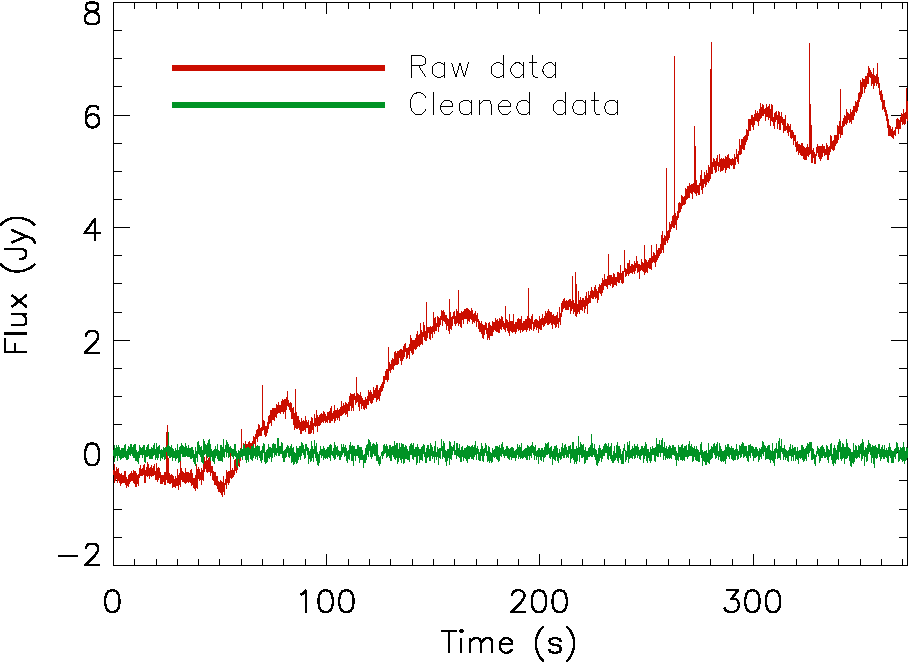
\includegraphics[height=6cm]{Figure/TOI_real}
	\hspace*{0.5cm}
	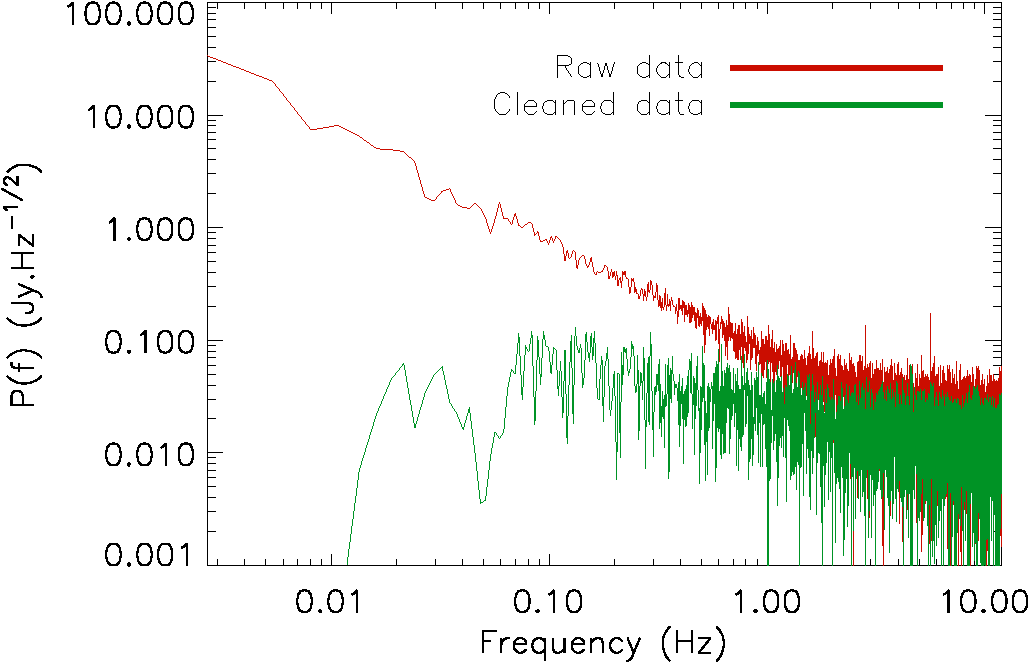
\includegraphics[height=6cm]{Figure/PS_real}
	\caption{TOD (left) and their power spectra (right) for a given detector. The data corresponds to the calibrated TOD before (red) and after (green) the electronic and atmospheric noise decorrelation. The TOD are dominated by the atmospheric noise at low frequencies, which is responsible for the slow variations in the red TOD and the obvious rise of noise below $\sim 1$~Hz on the red power spectrum. Cosmic rays hitting the instrument can be seen as spikes in the TOD but have been removed before computing the power spectra. Pulse tube frequency lines appear in the power spectrum ({\it e.g.} the $\sim 6$~Hz line in the raw power spectrum) and are notch filtered. The electronic noise dominates at frequencies between $\sim 1$ and $\sim 5$~Hz in the power spectrum before decorrelation.} \label{fig:TOI_PS_real}
	\end{figure*}
The main steps for processing the time ordered data (TOD) are listed below.
\begin{itemize}
\item Loading raw data, including the telescope parameters, the reconstruction of the projection of the array on the sky, and the atmospheric opacity.
\item Calibrating the TOD, including opacity correction.
\item Flagging invalid detectors.
\item Flagging cosmic ray impacts on the detectors.
\item Decorrelating atmospheric and electronic noise.
\item Filtering low frequencies and removing lines produced by the pulse tube of the cryostat with a notch filter.
\item Making map using inverse variance weighting.
\end{itemize}
In the following, we give details on specific points of the analysis.

\subsubsection{Raw data}
The raw TOD correspond to the real ($I_k(t)$, in-phase) and imaginary ($Q_k(t)$, quadrature) parts of the transfer function of the system (array and transmission line), which are sampled on predefined frequency tones $k$ at an acquisition rate of 23.842~Hz. We also compute the average modulation of these quantities with respect to the injected frequency (typically a few~kHz), which are noted $\delta I_k(t)$ and $\delta Q_k(t)$. These four quantities are used to reconstruct the shift of the resonance frequency ${\delta f_0}_k (t)$, which probes the optical power absorbed by a detector \citep[see][for more details]{RFdIdQ}. To monitor the electronic noise and possible variations of the transfer function of the transmission line, the latter is also sampled with tones that are placed off-resonance (with no correspondence to any detector), which are insensitive to optical power.

In the case of the {\it NIKA} prototype, some detectors are subject to cross talk and are not used for this analysis. Bad detectors are also flagged on the basis of the statistical properties of their noise. In particular, we use skewness and kurtosis tests, in addition to testing the stationarity of the noise. Some TODs, which are affected by baseline jumps due to the coupling with ambient magnetic fields, are also excluded. These rejected detectors are not used in the following. For the observations of \mbox{RX~J1347.5-1145}, the number of detectors used in the analysis is 81 at 140~GHz and 45 at 240~GHz.

\subsubsection{Calibration}
The shift of the resonance frequency is computed for each detector. The absolute calibration from resonance frequency to flux density is applied to these TODs. The beam is measured with Uranus observations in atmospheric conditions that are similar to those for the \mbox{RX~J1347.5-1145} observations. The Uranus data are fitted with a Gaussian function of FWHM that is equal to 12.5 and 18.5~arcsec at 240 and 140~GHz, respectively. An opacity correction is performed by multiplying the data by $\mathrm{exp}\left( \tau_{\nu_b} / \mathrm{sin}(el) \right)$, where $el$ is the elevation of the source. The calculation of the opacity is based on skydip measurements, as briefly described in Sect.~\ref{sec:calib_pointing} \cite[for more details, see][]{main_run5}.

\subsubsection{Glitch removal}
Cosmic rays hitting the instrument induce glitches in the data. The time response of KIDs is negligible compared to the sampling frequency, such that a cosmic ray impact appears as a peak on a single data sample in the TOD. We detect about four glitches per minute. They are removed from the ${\delta f_0}_k (t)$ TODs by flagging peaks that are above five times the standard deviation of the considered TOD. The TODs are flagged and interpolated at the glitch locations in order not to affect the decorrelation. These flagged data are not projected onto maps. 

\subsubsection{Dual-band decorrelation}
\label{sec:2band_decor}
As discussed above the atmospheric contribution to the NIKA data, $A(\nu_b, t)$, is essentially due to water vapor, to first order. Therefore, it is expected to be the same for the two frequency bands up to an amplitude factor $A(240~\mathrm{GHz},~t)/A(140~\mathrm{GHz},~t)~\simeq~5$. As a consequence, we first use the 240~GHz data to build an atmospheric template and remove it from the 140~GHz data by linear fitting. The fit is performed  for each subscan and for each 140~GHz detector independently. As the tSZ signal at 240~GHz is smaller by a factor of 5.5 (see  unit conversion factors between Compton parameter and Jansky per beam  in Sect.~\ref{sec:tsz_data}) with respect to the one at the 140~GHz band, the positive bias introduced in the 140~GHz data by the tSZ signal present at 240~GHz is negligible (about 27 times smaller). 

As shown in the left panel of Figure~\ref{fig:TOI_PS_real}, where we present the raw TOI signal for a typical KID at 140~GHz in red, the atmospheric contribution is dominated by a low frequency component. These drifts correspond to the $1/f$ noise-like spectrum with a knee frequency at about 1~Hz, which is presented in red on the right panel of the figure. We thus apply a low-pass filter to the atmospheric template that is deduced from the 240~GHz channel. This filter removes most of the detector correlated electronic noise in the 240~GHz band, $E(240 \ \mathrm{GHz}, t)$, which does not affect the 140~GHz data.  Furthermore, it allows us to reduce the intrinsic high noise level of the 240~GHz band, which was specific to the November 2012 {\it NIKA} data due to the cold amplifier disfunction and would otherwise pollute the 140~GHz cleaned data. The low-pass filter does not affect frequencies smaller than 1.5~Hz and sets frequencies larger than 2~Hz to zero. Frequencies between 1.5 and 2~Hz are progressively attenuated using a cosine squared cutoff. 

We also build a template from a high-pass filtered common-mode obtained from the TODs of the valid 140GHz detectors. This high-pass filter is the complement to the previous low-pass filter such that their sum is equal to one for all frequencies. We linearly fit this template to each subscan of each 140GHz detector TOD and remove it. As a consequence the correlated electronic noise, $E(140 \ \mathrm{GHz}, t)$ is removed at frequencies larger than the cutoff. We note that this does not significantly affect the tSZ signal because it is not correlated at these high frequencies between detectors as they observe different positions on the sky. Typically, 2~Hz corresponds to about 8~arcsec for the chosen scan speed (about 15~arcsec per second).

Finally, we fit and remove a template that follows the elevation of the telescope from the TODs. Indeed, as the oxygen component of the atmosphere is ignored in the dual-band decorrelation, it appears as a residual proportional to the elevation of the telescope.  \\

The main drawback of the dual-band decorrelation technique is the possible contamination of the 140~GHz tSZ reconstructed signal by other astrophysical components present at 240~GHz. First, we consider the kinematic Sunyaev-Zel'dovich (kSZ) effect, which is due to the overall motion of a cluster (or its components) with respect to the CMB reference frame and follows a pure black-body spectrum at the CMB temperature. The kSZ signal is also reduced by a factor of $\sim 5$, such that its flux at 240~GHz should be larger than half the tSZ flux at 140~GHz to produce a non-negligible bias. This is not the case even for the most extreme clusters, such as \mbox{MACS~J0717.5+3745}~\citep{mroczkowski_2012, sayers2013}. Therefore, any kSZ signal present at 240~GHz is neglected in the following analysis.

We have also searched for dusty galaxies within the cluster or gravitationally lensed submilimeter high-redshift background objects that might also contaminate the signal at 140 and 240~GHz. As mentioned in Sect.~\ref{sec:previous_obs}, two of such sources are present in \mbox{RX~J1347.5-1145}. Despite the high level of noise in the 240~GHz {\it NIKA} data for this campaign, the first source, Z1, (R.A,~Dec)~=~(13h~47m~27.6s,~-11$^{\mathrm{o}}$~45'~54") is observed in this band with a flux of 12.7 mJy $\pm$ 6.2. The second source, Z2, (R.A,~Dec)~=~(13h~47m~31.3s,~-11$^{\mathrm{o}}$~44'~57") is not detected in the 240~GHz {\it NIKA} band, but we obtain an upper limit of 4.4 mJy at 1 $\sigma$. Using this information and the measured fluxes at 850 and 450~$\mu$m (see Sect.~\ref{sec:previous_obs}), we estimate the expected flux of the sources at 140~GHz. Assuming dust temperatures in the range of 15 -- 20 K and dust spectral indexes $\beta_{\mathrm{d}}$ in the range of 1.5 -- 2, we obtain 0.85 mJy  at 140~GHz for the Z1 source. For the second source, Z2, we are not able to fit a typical dust spectrum and only compute an upper limit of the flux at 140~GHz by assuming a Rayleigh-Jeans spectrum at low frequency and using the 240~GHz estimated flux. We obtain an upper limit at 140~GHz of 0.65 mJy. In the context of dual-band decorrelation, the 240~GHz fluxes are scaled down by $\simeq 5$, and they are diluted by another factor of $\simeq 5$ due the averaging over all the 240~GHz detectors, which observe the source at different time samples. As uncertainties on the estimated flux for both sources and at both wavelengths are large, we choose not to subtract them directly in the TOD but to account for them in the final analysis, as discussed in Sect.~\ref{sec:ps_sub_effect}.

\subsubsection{Fourier filtering}
Frequency lines ({\it e.g.} at $\sim$ 6~Hz) are induced by the pulse tube of the cryostat and observed in the TOD power spectra (see Fig.~\ref{fig:TOI_PS_real}, right panel). They are flagged and set to zero. In addition, we apply a high-pass filter to remove correlated noise at frequencies lower than the subscan because no tSZ signal is present there. We also remove low frequency (below 0.05~Hz) sine and cosine from the data to further subtract correlated noise contamination.

\subsection{Mapmaking}
\label{sec:mapmaking}
Finally, we construct surface brightness maps by projecting and averaging the signal from all KIDs on a pixelized map at 140~GHz. The projected data are weighted according to the level of noise of each detector using inverse variance weighting. To remove possible offsets in the TOD, we subtract the mean value of each TODs, and we take the zero level as the mean of the external part of the map, where no signal is detected.
	
\subsection{Point source subtraction}
\label{sec:point_source}
The object RX~J1347.51145 hosts a radio point source located within 3~arcsec of the X-ray center that has a flux of $4.4 \pm 0.3$~mJy and $3.2 \pm 0.2$~mJy  at 140 and 240~GHz, respectively~\citep{pointecouteau_2001}. The point source is subtracted in the TODs at both frequencies before the processing, so that it does not bias the analysis. We discuss in Sect.~\ref{sec:ps_sub_effect} how uncertainties on the point source subtraction affect the final results.

